\section{Theoretical Foundations}
\label{sec:Theoretical_Foundations}
This section summarizes the theory and formulas necessary to understand the following experiments on interference and diffraction in section \ref{sec:Evaluation}.

\subsection{Wave Interference}
\label{subsec:Interference}
Interference is caused, when two waves superpose to form a wave of greater, lower or the same amplitude. The interfering waves are usually coherent with each other, either because they come from the same source or because they have the same frequency \cite{diffraction}.

\subsection{Diffraction Slit / Anti-Slit}
\label{subsec:Diffraction_Slit}
The minima of the diffraction pattern of a slit or an anti-slit $\varphi_m$ can be derived by using the Huygens–Fresnel principle. It states that every point on a slit is itself the source of spherical wavelets. These wavelets have the same amplitude and phase \cite{diffraction}.

The order $m$, the wavelength $\lambda$ and the width of the slit $w$ is used to calculate the minima $\varphi_m$:
\begin{equation}
\sin\varphi_m = \frac{m\cdot\lambda}{w} \qquad \text{with} \qquad m = \pm 1, \pm 2, ...
\label{eq:slit_minima}
\end{equation}
To obtain the maxima $\varphi_m$, the following equation is used \cite{uni_hamburg}:
\begin{equation}
\sin\varphi_m =
\begin{cases} 
	0 & \qquad \text{for} \qquad m = 0\\
	\left(m + \frac{1}{2}\right)\cdot\frac{\lambda}{w} & \qquad \text{for} \qquad m = 1, 2, 3, ...\\[6pt]
	\left(m - \frac{1}{2}\right)\cdot\frac{\lambda}{w} & \qquad \text{for} \qquad m = -1, -2, -3, ...
\end{cases}
\label{eq:slit_maxima}
\end{equation}
where:
\begin{conditions}
	\varphi_m & angle of the interference of order $m$ \\
	m & order of the interference \\
	\lambda & wavelength of the laser \\
	w & width of the slit or the anti-slit
\end{conditions}
\begin{figure}[H]
	\centering
	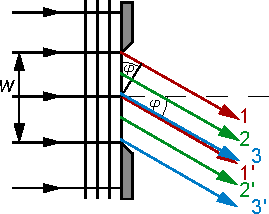
\includegraphics[scale=1.5]{slit_theory}
	\caption{Diffraction of light on a slit \cite{diffraction} - partially modified}
	\label{fig:diff_slit}
\end{figure}
Figure \ref{fig:diff_slit} shows the diffraction of light on a slit. The partial wave 1 (red) and the partial wave 2 (green) differ by $\lambda/2$ and thus interfere destructively, which results in a minimum. The width of the slit is denoted as $w$ and the angle of interference is denoted as $\varphi$ \cite{diffraction}.

\subsection{Diffraction Circular Aperture}
\label{subsec:Diffraction_Circular_Aperture}
When diffraction occurs at a circular aperture, interference rings can be observed. The angles at which the minima occur can be derived by using the following equation \cite{diffraction}:
\begin{equation}
\sin\varphi_c = \frac{c_k\cdot\lambda}{d} \qquad \text{with} \qquad c_k = \frac{j_{\text{1,k}}}{\pi}
\label{eq:circular_aperture}
\end{equation}
The first five Bessel coefficients $c_k$ are the following (used in this laboratory report):
\begin{equation}
c_k = \{1.220,~2.233,~3.238,~4.241,~5.243,~...\}
\label{eq:coeffs}
\end{equation}
where:
\begin{conditions}
	\varphi_c & angle of the interference \\
	c_k & order of the interference \\
	j_{\text{1,k}} & $k$th positive zero of the Bessel function $J_1(x)$ \\
	\lambda & wavelength of the laser \\
	d & diameter of the circular aperture
\end{conditions}
The Bessel coefficients $c_k$ shown above were calculated with MATLAB (see appendix \ref{sec:MATLAB_Error_Calculation}).

\subsection{Diffraction Cross-Grid Aperture}
\label{subsec:Diffraction_Cross-Grid_Aperture}
To calculate the maximas of a cross-grid aperture on either the x-axis or the y-axis, the equation for a line-grid can be used \cite{diffraction}.
\begin{equation}
\sin\varphi_m = \frac{m\cdot\lambda}{g}
\label{eq:cross-grid}
\end{equation}
where:
\begin{conditions}
	\varphi_m & angle of the interference of order $m$ \\
	m & order of the interference \\
	\lambda & wavelength of the laser \\
	g & grid constant
\end{conditions}
For the above equation \ref{eq:cross-grid} to be valid, the distance between the cross-grid aperture and the projection surface ($x$) must be large \cite{diffraction}.
\begin{figure}[H]
	\centering
	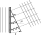
\includegraphics[scale=1.5]{line-grid}
	\caption{Diffraction of light on a line-grid \cite{diffraction} - partially modified}
	\label{fig:line-grid}
\end{figure}
Figure \ref{fig:line-grid} shows the diffraction of light on a line-grid, which is a simplified version of the cross-grid. The angle of interference is denoted as $\varphi$.

\subsection{Calculation of the Angle $\varphi$}
\label{subsec:Calculation_of_the_Angle}
The angle of the interference $\varphi$ is only measured indirectly by measuring the distance from the aperture to the projection surface ($x$) and the position of the maxima or minima ($y$).
\begin{figure}[H]
	\centering
	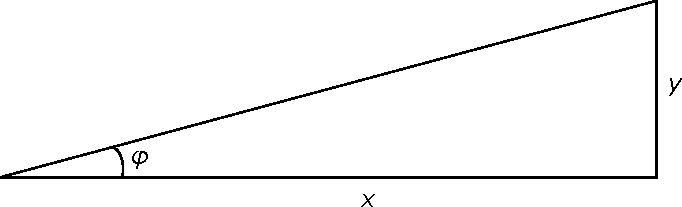
\includegraphics[scale=1]{angle}
	\caption{Calculation of the angle $\varphi$}
	\label{fig:angle}
\end{figure}
Figure \ref{fig:angle} shows the relationship between the angle $\varphi$ and the distances $x$ and $y$. To calculate the angle of interference the following equation \ref{eq:angle} is used:
\begin{equation}
\varphi = \arctan\left(\frac{y}{x}\right)
\label{eq:angle}
\end{equation}
where:
\begin{conditions}
	\varphi & angle of the interference \\
	$x$ & distance between the aperture and the projection surface (see figure \ref{fig:experimental_arrangement}) \\
	$y$ & position of the maxima or the minima
\end{conditions}
